\documentclass[10.5pt,oneside]{article}

% -------------------- page and typography --------------------
\usepackage[letterpaper,margin=0.78in,top=0.72in,bottom=0.78in]{geometry}
\usepackage[T1]{fontenc}
\usepackage[utf8]{inputenc}
\usepackage{newtxtext}
\usepackage{microtype}
\usepackage{setspace}
\usepackage{parskip}
\usepackage{enumitem}
\usepackage{booktabs}
\usepackage{array}
\usepackage{tabularx}
\usepackage{longtable}
\usepackage{ragged2e}
\usepackage{multicol}
\usepackage{xcolor}
\usepackage{tikz}
\usepackage[most]{tcolorbox}
\usepackage{titlesec}
\usepackage{fancyhdr}
\usepackage{lastpage}
\usepackage{hyperref}
\usepackage{caption}
\usepackage{adjustbox}
\usepackage{float}
\usepackage{listings}
\usepackage{amsmath}
\usepackage{etoolbox}

\usetikzlibrary{arrows.meta,positioning,calc,fit,backgrounds,shapes.geometric,shapes.misc,decorations.pathreplacing,patterns,shadows.blur}

% -------------------- color system --------------------
\definecolor{Navy}{HTML}{071A4C}
\definecolor{Ink}{HTML}{10141F}
\definecolor{Muted}{HTML}{5E667B}
\definecolor{Violet}{HTML}{5B3FD6}
\definecolor{Violet2}{HTML}{8E75FF}
\definecolor{Cyan}{HTML}{37C8F4}
\definecolor{Gold}{HTML}{B88423}
\definecolor{Gold2}{HTML}{E3B14B}
\definecolor{Green}{HTML}{15845E}
\definecolor{Red}{HTML}{B33A4B}
\definecolor{Amber}{HTML}{F2A93B}
\definecolor{Plate}{HTML}{FBFAF6}
\definecolor{Plate2}{HTML}{F2F6FF}
\definecolor{DarkPlate}{HTML}{0B1024}
\definecolor{Line}{HTML}{D9D2C2}

\hypersetup{
  colorlinks=true,
  linkcolor=Navy,
  citecolor=Violet,
  urlcolor=Violet,
  pdftitle={GoalOS: The Validated Skill Graph},
  pdfauthor={Montreal.AI Research},
  pdfsubject={Reusable capability, Chronicle-gated memory, proof-carrying skill accumulation},
  pdfkeywords={GoalOS, Validated Skill Graph, ProofBundles, Evidence Docket, Chronicle Gate, reusable capability, AGI Jobs}
}

\setstretch{1.05}
\emergencystretch=3em
\setlist[itemize]{leftmargin=1.2em,itemsep=0.22em,topsep=0.35em}
\setlist[enumerate]{leftmargin=1.4em,itemsep=0.25em,topsep=0.35em}

\titleformat{\section}
  {\Large\bfseries\scshape\color{Navy}}
  {\thesection}{0.55em}{}
  [\vspace{0.18em}{\color{Gold}\titlerule[0.7pt]}]
\titleformat{\subsection}
  {\normalsize\bfseries\color{Navy}}
  {\thesubsection}{0.55em}{}
\titleformat{\subsubsection}
  {\normalsize\bfseries\itshape\color{Ink}}
  {\thesubsubsection}{0.55em}{}

\setlength{\headheight}{20pt}
\pagestyle{fancy}
\fancyhf{}
\lhead{\small\scshape GoalOS: The Validated Skill Graph}
\rhead{\small\scshape Montreal.AI Research}
\cfoot{\small\color{Navy}\thepage\,/\,\pageref*{LastPage}}
\renewcommand{\headrulewidth}{0.35pt}
\renewcommand{\headrule}{\hbox to\headwidth{\color{Gold}\leaders\hrule height \headrulewidth\hfill}}

\captionsetup{font=small,labelfont={bf,color=Navy},labelsep=period}

% -------------------- code blocks --------------------
\lstdefinestyle{jsonstyle}{
  basicstyle=\ttfamily\small,
  backgroundcolor=\color{Plate2},
  frame=single,
  rulecolor=\color{Line},
  breaklines=true,
  showstringspaces=false,
  columns=fullflexible,
  tabsize=2,
  xleftmargin=0.5em,
  xrightmargin=0.5em
}

% -------------------- reusable boxes and tikz styles --------------------
\newtcolorbox{thesisbox}{
  enhanced,
  colback=Plate,
  colframe=Gold,
  boxrule=0.7pt,
  arc=2.5mm,
  left=4mm,right=4mm,top=3mm,bottom=3mm,
  borderline west={2.2pt}{0pt}{Gold},
  before skip=0.8em, after skip=0.8em
}

\newtcolorbox{figureplate}{
  enhanced,
  colback=Plate,
  colframe=Line,
  boxrule=0.6pt,
  arc=3mm,
  left=2mm,right=2mm,top=2mm,bottom=2mm,
  before skip=0.5em, after skip=0.3em
}

\newcommand{\goalos}{\textsc{GoalOS}}
\newcommand{\vsg}{\textsc{Validated Skill Graph}}
\newcommand{\chronicle}{\textsc{Chronicle}}
\newcommand{\proofbundle}{\textsc{ProofBundle}}
\newcommand{\evidencedocket}{\textsc{Evidence Docket}}
\newcommand{\agijob}{\textsc{AGI Job}}
\newcommand{\skillnode}{\textsc{SkillNode}}

\tikzset{
  flowarrow/.style={-{Latex[length=2.4mm,width=1.8mm]}, line width=0.75pt, draw=Violet},
  greenarrow/.style={-{Latex[length=2.4mm,width=1.8mm]}, line width=0.75pt, draw=Green},
  goldarrow/.style={-{Latex[length=2.2mm,width=1.6mm]}, line width=0.65pt, draw=Gold, dashed},
  redarrow/.style={-{Latex[length=2.2mm,width=1.6mm]}, line width=0.65pt, draw=Red},
  softnode/.style={rounded corners=6pt, draw=Violet!45, fill=white, line width=0.55pt, align=center, inner sep=5pt, font=\footnotesize},
  cardnode/.style={rounded corners=7pt, draw=Navy!25, fill=Plate2, line width=0.55pt, align=center, inner sep=6pt, font=\footnotesize},
  gatenode/.style={diamond, aspect=2, draw=Gold!80!black, fill=Gold!10, line width=0.7pt, align=center, inner sep=2pt, font=\scriptsize\bfseries},
  skillcircle/.style={circle, draw=Violet!50, fill=white, line width=0.65pt, minimum size=1.35cm, align=center, font=\scriptsize},
  darkbox/.style={rounded corners=6pt, draw=Violet2!60, fill=DarkPlate, text=white, line width=0.6pt, align=center, inner sep=5pt, font=\scriptsize},
  labeltiny/.style={font=\scriptsize, align=center, text=Navy},
}

% -------------------- document --------------------
\begin{document}

% ==================== title page ====================
\begin{titlepage}

\begin{tikzpicture}[remember picture,overlay]
  \fill[DarkPlate] (current page.south west) rectangle (current page.north east);
  \foreach \i in {0,...,26}{
    \draw[white,opacity=0.025,line width=0.2pt] ($(current page.south west)+(0,\i*0.42)$) -- ($(current page.south east)+(0,\i*0.42)$);
  }
  \foreach \i in {0,...,18}{
    \draw[white,opacity=0.025,line width=0.2pt] ($(current page.south west)+(\i*0.45,0)$) -- ($(current page.north west)+(\i*0.45,0)$);
  }
  \draw[Gold2,opacity=0.75,line width=0.7pt] ($(current page.north west)+(0.75,-0.75)$) -- ($(current page.north east)+(-0.75,-0.75)$);
  \draw[Gold2,opacity=0.75,line width=0.7pt] ($(current page.south west)+(0.75,0.75)$) -- ($(current page.south east)+(-0.75,0.75)$);
  \begin{scope}[shift={(current page.center)}, opacity=0.55]
    \draw[Violet2,line width=0.5pt] (0,0) circle (4.3);
    \draw[Cyan,line width=0.5pt, opacity=0.42] (0,0) circle (3.0);
    \draw[Gold,line width=0.6pt, opacity=0.45] (-3.55,0) -- (3.55,0);
    \draw[Gold,line width=0.6pt, opacity=0.45] (0,-3.55) -- (0,3.55);
    \foreach \ang in {0,45,...,315}{\draw[Violet2,opacity=0.5] (0,0) -- (\ang:4.3);}
    \foreach \ang/\r in {25/4.3,105/3,190/4.3,250/3,310/4.3}{\fill[Gold2,opacity=0.9] (\ang:\r) circle (1.2pt);}
  \end{scope}
\end{tikzpicture}
\vspace*{1.2cm}
\begin{center}
  {\color{Gold2}\Large\scshape Montreal.AI Research}\par\vspace{1.4cm}
  {\color{white}\fontsize{35}{39}\selectfont\bfseries GoalOS:\ The Validated Skill Graph}\par\vspace{0.35cm}
  {\color{Cyan!85}\fontsize{16}{20}\selectfont Reusable Capability, Chronicle-Gated Memory, and Proof-Carrying Skill Accumulation}\par\vspace{1.2cm}
  \begin{tcolorbox}[enhanced,width=0.86\textwidth,colback=white!6!DarkPlate,colframe=Gold2!70,boxrule=0.6pt,arc=3mm,left=5mm,right=5mm,top=4mm,bottom=4mm]
  {\color{white}\large\itshape
  The durable asset is not the prompt. It is the proof-carrying skill node. The durable advantage is not more output. It is a graph of validated capability that can be reused, composed, taught, packaged, audited, retired, and trusted.}
  \end{tcolorbox}
  \vfill
  {\color{white!72}\small Publication-safe, claim-bounded research edition.}\par
  {\color{white!72}\small July 2026}\par
\end{center}
\end{titlepage}

\pagenumbering{arabic}

\begin{center}
{\LARGE\bfseries GoalOS: The Validated Skill Graph}\par
\vspace{0.25em}
{\large\itshape Reusable Capability, Chronicle-Gated Memory, and Proof-Carrying Skill Accumulation}\par
\vspace{0.6em}
{\scshape Montreal.AI Research}\par
\vspace{0.8em}
{\color{Gold}\rule{0.72\linewidth}{0.6pt}}\par
\end{center}

\begin{abstract}
\noindent
This paper introduces the \vsg{}: a proof-carrying memory substrate for autonomous AI work. Conventional AI memory stores text, embeddings, prompts, or traces. Such memory is easy to accumulate but difficult to govern; it may preserve persuasive output without evidence, replay, risk context, or admission policy. The \vsg{} treats reusable capability as a typed, scoped, versioned, evidence-backed object. A candidate skill may originate from an LLM draft, an expert intervention, an AGI Job, a reviewer critique, or a repeated mission pattern, but it cannot influence future missions until it passes a \chronicle{} admission gate. Admission requires an \evidencedocket{}, returned \proofbundle{} artifacts, proof-level-dependent acceptance checks, risk posture, replay or reconstruction path, and a rollback condition. Accepted nodes become reusable capability; rejected or partial nodes become repair paths or custom AGI Jobs. We formalize the skill node object model, graph operations, proof-level policy ladder, worth-keeping utility, threat model, and evaluation program. The central claim is architectural: compounding value in a proof economy does not come from larger prompt libraries; it comes from validated skill graphs that convert proof-bearing work into governed, reusable, and auditable capability.
\end{abstract}

\begin{thesisbox}
\textbf{Thesis.} \goalos{} creates proof; the \vsg{} makes proof reusable. A model may draft, an agent may act, and a reviewer may validate, but only a \chronicle{}-admitted skill node may influence future missions.
\end{thesisbox}

\section{Introduction}
The first wave of AI systems made generation abundant. They produced text, plans, code, reports, search results, and agent traces at low marginal cost. Abundance, however, is not the same as institutional trust. An organization does not merely need to remember what an agent said; it needs to know which outputs deserve reuse, payment, propagation, training, settlement, and rollback authority.

The \vsg{} addresses this missing layer. It is not a prompt repository, vector database, note archive, or transcript store. It is a governed capability graph. Nodes are validated skills; edges describe how those skills can be reused, composed, taught, packaged, audited, retired, or applied to future missions. The graph is populated only through \chronicle{} admission: a policy gate that checks evidence, replay, validation, risk, and scope. This transforms memory from an informal convenience into an institutional control surface.

The design follows the \goalos{} proof loop: an objective becomes a mission contract; unsupported claims become proof debt; proof debt becomes custom AGI Jobs; jobs return \proofbundle{} artifacts; artifacts enter an \evidencedocket{}; the \chronicle{} gate decides what becomes durable memory; admitted nodes become reusable capability. The \vsg{} is therefore the compounding layer of the proof economy.

\section{Problem Statement: Memory Without Proof}
Ungated AI memory creates four recurring failures.

\begin{enumerate}
  \item \textbf{Contamination.} A persuasive but unsupported answer can shape future behavior if it is stored as memory.
  \item \textbf{Drift.} Instructions, heuristics, or tactics copied across runs lose context and gradually exceed their original scope.
  \item \textbf{Irreplayability.} A remembered result may not include inputs, methods, versions, reviewers, or artifacts sufficient to reconstruct it.
  \item \textbf{Authority leakage.} A local draft may be mistaken for validated evidence, settlement readiness, or production permission.
\end{enumerate}

These failures are not solved by larger context windows or better summaries. They require a memory object with admission policy, provenance, versioning, evidence linkage, and rollback. The \vsg{} supplies this object.

\section{System Positioning}
The \vsg{} is one layer in a larger proof economy. It receives candidates from human experts, LLMs, AGI Agents, reviewers, and mission traces, but it is not controlled by any one of them. Its authority comes from the \chronicle{} gate.

\begin{itemize}
  \item A \textbf{prompt repository} stores instruction fragments. A \textbf{validated skill graph} stores evidence-backed capability.
  \item A prompt can be copied. A validated skill carries provenance, acceptance tests, scope, and rollback.
  \item A prompt can drift. A skill node has versioned constraints and an explicit admissible-use envelope.
  \item A prompt may persuade. A skill node must survive proof.
\end{itemize}

\begin{figure}[H]
\centering
\begin{figureplate}
\centering
\resizebox{0.98\textwidth}{!}{%
\begin{tikzpicture}[x=1cm,y=1cm]
\path[use as bounding box] (0,0) rectangle (15.8,9.2);
\fill[Plate2,rounded corners=11pt] (0.05,0.05) rectangle (15.75,9.15);
\draw[Line,rounded corners=11pt,line width=0.55pt] (0.05,0.05) rectangle (15.75,9.15);

% title bands
\node[font=\bfseries\color{Navy}] at (7.9,8.72) {Validated Skill Graph as Proof-Gated Capability Memory};
\draw[Gold,line width=0.45pt] (4.2,8.45) -- (11.6,8.45);

% four strata panels
\foreach \x/\title/\sub in {1.9/{Candidate Work}/{Drafts, traces, expert moves},5.55/{Proof Economy}/{Jobs, bundles, evidence},9.25/{Chronicle Gate}/{Admission and repair},13.0/{Validated Memory}/{Reusable capability}}{
  \draw[Navy!18,fill=white,rounded corners=8pt] (\x-1.6,5.0) rectangle (\x+1.6,8.0);
  \node[font=\bfseries\scriptsize\color{Navy},align=center] at (\x,7.72) {\title};
  \node[font=\scriptsize\color{Muted},align=center] at (\x,7.38) {\sub};
}

% candidate work
\node[softnode,minimum width=1.8cm] (draft) at (1.9,6.8) {LLM / Expert\\candidate};
\node[softnode,minimum width=1.8cm] (claim) at (1.9,5.95) {Claim\\extraction};
\node[softnode,minimum width=1.8cm] (debt) at (1.9,5.10) {Proof debt\\items};
\draw[flowarrow] (draft) -- (claim);
\draw[flowarrow] (claim) -- (debt);

% proof economy
\node[softnode,minimum width=2.1cm] (jobs) at (5.55,6.65) {Custom\\AGI Jobs};
\node[softnode,minimum width=2.1cm] (pb) at (5.55,5.80) {ProofBundles};
\node[softnode,minimum width=2.1cm] (ed) at (5.55,4.95) {Evidence\\Docket};
\draw[flowarrow] (jobs) -- (pb);
\draw[flowarrow] (pb) -- (ed);
\draw[flowarrow] (debt.east) -- (jobs.west);

% gate
\node[gatenode,minimum width=2.2cm] (gate) at (9.25,5.9) {Chronicle\\Gate};
\node[cardnode,minimum width=2.25cm,fill=Green!8,draw=Green!40] (admit) at (9.25,7.10) {Admit\\validated node};
\node[cardnode,minimum width=2.25cm,fill=Gold!9,draw=Gold!55] (repair) at (9.25,4.75) {Repair\\create jobs};
\node[cardnode,minimum width=2.25cm,fill=Red!6,draw=Red!45] (reject) at (9.25,3.75) {Reject or\\quarantine};
\draw[flowarrow] (ed.east) -- (gate.west);
\draw[greenarrow] (gate) -- (admit);
\draw[goldarrow] (gate) -- (repair);
\draw[redarrow] (gate) -- (reject);
\draw[goldarrow] (repair.west) .. controls (7.7,4.05) and (6.7,4.1) .. (jobs.south);

% memory graph
\node[skillcircle,minimum size=1.62cm,fill=white] (core) at (13.05,5.55) {Validated\\Skill\\Graph};
\foreach \ang/\lab in {90/Reuse,25/Compose,-35/Teach,-90/Package,-155/Audit,155/Replay}{
  \node[skillcircle,minimum size=0.96cm] (n\ang) at ($(core)+(\ang:1.25)$) {\lab};
  \draw[flowarrow] (core) -- (n\ang);
  \draw[flowarrow] (n\ang) -- (core);
}
\draw[greenarrow] (admit.east) -- (core.west);
\draw[goldarrow] (core.south) .. controls (12.2,2.55) and (2.7,2.4) .. node[below,midway,font=\scriptsize\color{Gold!80!black}]{future mission influence only from admitted skills} (draft.south);

% bottom law
\draw[Gold!55,rounded corners=5pt,fill=white] (0.75,0.65) rectangle (15.05,1.35);
\node[align=center,font=\footnotesize] at (7.9,1.0) {\textbf{Memory law.} Drafts may propose; only proof-admitted skills persist. Failed candidates repair proof debt, not memory.};

% legend
\draw[flowarrow] (1.1,2.0) -- (2.0,2.0); \node[anchor=west,font=\scriptsize] at (2.08,2.0) {control flow};
\draw[greenarrow] (4.0,2.0) -- (4.9,2.0); \node[anchor=west,font=\scriptsize] at (4.98,2.0) {validated memory commit};
\draw[goldarrow] (7.2,2.0) -- (8.1,2.0); \node[anchor=west,font=\scriptsize] at (8.18,2.0) {repair / future influence};
\draw[redarrow] (11.0,2.0) -- (11.9,2.0); \node[anchor=west,font=\scriptsize] at (11.98,2.0) {reject path};
\end{tikzpicture}}
\end{figureplate}
\caption{The \vsg{} as a governed memory substrate. Candidate work becomes durable capability only after proof, evidence aggregation, and \chronicle{} admission.}
\label{fig:substrate}
\end{figure}

Figure~\ref{fig:substrate} positions the \vsg{} as a memory substrate rather than a convenience layer. Drafts, traces, and expert moves remain outside durable memory until they become evidence-backed skill nodes.

\section{Formal Object Model}
A skill node is a scoped capability record. It contains not only a description of what worked, but the conditions under which the capability may be used again. Formally, a skill node is:
\[
  s = \langle id, type, scope, method, evidence, tests, validators, risk, policy, version, rollback, utility \rangle.
\]

\noindent The fields have the following interpretation.
\begin{description}[leftmargin=2.2cm,style=nextline]
\item[\texttt{id}] A stable identifier bound to mission lineage, version, and content hash.
\item[\texttt{type}] The role of the skill: vision-to-proof, domain research, reviewer judgment, job design, replay, boundary audit, or composite skill.
\item[\texttt{scope}] The admissible-use envelope: domain, assumptions, proof level, jurisdiction, tools, and excluded uses.
\item[\texttt{method}] The procedure, heuristics, toolchain, and sequencing that produced the result.
\item[\texttt{evidence}] Links to \proofbundle{} artifacts, \evidencedocket{} entries, replay manifests, reviewer notes, and metrics.
\item[\texttt{tests}] Acceptance tests required before reuse or composition.
\item[\texttt{validators}] Human, AGI Node, council, or hybrid validators, including review state and quorum.
\item[\texttt{risk}] Risk posture, failure modes, open debt, and repair conditions.
\item[\texttt{policy}] Admission level, reuse permissions, retention period, and mainnet handoff boundary.
\item[\texttt{version}] Version number, parent nodes, supersession path, and changelog.
\item[\texttt{rollback}] Conditions for demotion, quarantine, or retirement.
\item[\texttt{utility}] Estimated and measured contribution to future mission success, cost reduction, speed, trust, or safety.
\end{description}


\begin{figure}[H]
\centering
\begin{figureplate}
\centering
\resizebox{0.98\textwidth}{!}{%
\begin{tikzpicture}[x=1cm,y=1cm]
\path[use as bounding box] (0,0) rectangle (15.8,9.2);
\fill[Plate2,rounded corners=11pt] (0.05,0.05) rectangle (15.75,9.15);
\draw[Line,rounded corners=11pt,line width=0.55pt] (0.05,0.05) rectangle (15.75,9.15);
\node[font=\bfseries\color{Navy}] at (7.9,8.72) {Skill Node Object Model};
\draw[Gold,line width=0.45pt] (5.25,8.48)--(10.55,8.48);

% central node
\draw[rounded corners=9pt,fill=white,draw=Violet!45,line width=0.75pt,blur shadow={shadow blur steps=5,shadow blur extra rounding=2pt}] (5.95,5.55) rectangle (9.85,7.55);
\node[font=\bfseries\color{Navy},align=center] at (7.9,7.15) {Validated Skill Node};
\node[font=\scriptsize\color{Muted},align=center] at (7.9,6.83) {policy-bearing reusable capability};
\node[font=\footnotesize\color{Ink},align=center] at (7.9,6.30) {bounded capability\\with evidence, policy, and rollback};

% four schema quadrants
\node[cardnode,minimum width=3.45cm,minimum height=1.25cm,fill=white] (identity) at (2.55,5.95) {\textbf{Identity \& Scope}\\[-1pt]{\scriptsize id, type, domain, exclusions}};
\node[cardnode,minimum width=3.45cm,minimum height=1.25cm,fill=white] (method) at (2.55,3.85) {\textbf{Method \& Replay}\\[-1pt]{\scriptsize procedure, tools, tests, manifest}};
\node[cardnode,minimum width=3.45cm,minimum height=1.25cm,fill=white] (evidence) at (13.25,5.95) {\textbf{Evidence \& Validators}\\[-1pt]{\scriptsize ProofBundles, docket, reviewers}};
\node[cardnode,minimum width=3.45cm,minimum height=1.25cm,fill=white] (policy) at (13.25,3.85) {\textbf{Policy \& Lifecycle}\\[-1pt]{\scriptsize proof level, version, rollback}};

% no crossing: route via buses
\coordinate (leftbus) at (4.6,4.9);
\coordinate (rightbus) at (11.2,4.9);
\draw[flowarrow] (identity.east) -- ++(0.45,0) |- (6.0,6.65);
\draw[flowarrow] (method.east) -- ++(0.45,0) |- (6.0,6.15);
\draw[flowarrow] (evidence.west) -- ++(-0.45,0) |- (9.8,6.65);
\draw[flowarrow] (policy.west) -- ++(-0.45,0) |- (9.8,6.15);

% lifecycle path
\node[gatenode,minimum width=2.15cm] (gate) at (7.9,4.15) {Chronicle\\admission};
\node[cardnode,minimum width=2.8cm,fill=Green!8,draw=Green!45] (memory) at (7.9,2.65) {Durable skill\\memory entry};
\node[cardnode,minimum width=2.8cm,fill=Gold!10,draw=Gold!60] (repair) at (4.0,1.35) {Repair jobs\\if proof is missing};
\node[cardnode,minimum width=2.8cm,fill=Red!6,draw=Red!45] (retire) at (11.8,1.35) {Retire / rollback\\if policy fails};
\draw[flowarrow] (7.9,5.55) -- (gate.north);
\draw[greenarrow] (gate) -- (memory);
\draw[goldarrow] (gate.west) .. controls (6.4,3.0) and (5.0,2.0) .. (repair.north);
\draw[redarrow] (gate.east) .. controls (9.4,3.0) and (10.8,2.0) .. (retire.north);

% bottom law strip
\draw[Gold!65!black,fill=white,rounded corners=5pt] (1.0,0.35) rectangle (14.8,0.95);
\node[align=center,font=\footnotesize] at (7.9,0.65) {\textbf{Object law.} A skill node is a governed capability object: evidence-linked, scope-bound, replay-aware, versioned, and rollbackable.};
\end{tikzpicture}}
\end{figureplate}
\caption{A validated skill node contains operational semantics, evidence, policy, utility, and rollback. The node is a capability record, not a prompt fragment.}
\label{fig:node}
\end{figure}

\section{Chronicle Admission Policy}
\chronicle{} is the gate between evidence and memory. It is not a passive database write. A candidate skill enters the graph only if the configured proof level is satisfied. Let \(c\) be a candidate skill and \(\ell\) a proof level. The admission function is:
\[
 A_\ell(c) = \mathbf{1}\big[ E(c) \ge \tau^E_\ell \;\wedge\; R(c) \le \tau^R_\ell \;\wedge\; V(c) \ge \tau^V_\ell \;\wedge\; P(c)=1 \;\wedge\; B(c)=1 \big],
\]
where \(E\) measures evidence strength, \(R\) risk posture, \(V\) validation coverage, \(P\) replay or reconstruction readiness, and \(B\) boundary compliance. If \(A_\ell(c)=1\), the skill is admitted. If not, the system routes it to repair, rejection, quarantine, or further AGI Jobs.

\begin{figure}[H]
\centering
\begin{figureplate}
\centering
\resizebox{0.98\textwidth}{!}{%
\begin{tikzpicture}[x=1cm,y=1cm]
\path[use as bounding box] (0,0) rectangle (15.8,9.4);
\fill[Plate,rounded corners=11pt] (0.05,0.05) rectangle (15.75,9.35);
\draw[Line,rounded corners=11pt,line width=0.55pt] (0.05,0.05) rectangle (15.75,9.35);
\node[font=\bfseries\color{Navy}] at (7.9,8.92) {Chronicle Admission: Evidence Becomes Authority Only Through Policy};
\draw[Gold,line width=0.45pt] (4.2,8.67) -- (11.6,8.67);

\node[softnode,minimum width=2.35cm] (cand) at (1.6,5.2) {Candidate\\Skill};
\node[softnode,minimum width=2.35cm] (docket) at (4.1,5.2) {Evidence\\Docket};
\node[gatenode,minimum width=2.2cm] (gate) at (7.15,5.2) {Chronicle\\Gate};
\node[cardnode,minimum width=2.7cm,fill=Green!8,draw=Green!45] (admit) at (12.7,7.05) {Admit\\memory entry};
\node[cardnode,minimum width=2.7cm,fill=Gold!10,draw=Gold!60] (repair) at (12.7,5.2) {Repair\\custom AGI Jobs};
\node[cardnode,minimum width=2.7cm,fill=Red!6,draw=Red!45] (reject) at (12.7,3.35) {Reject or\\quarantine};
\draw[flowarrow] (cand) -- (docket);
\draw[flowarrow] (docket) -- (gate);
\draw[greenarrow] (gate) -- (admit);
\draw[goldarrow] (gate) -- (repair);
\draw[redarrow] (gate) -- (reject);

% four criteria around gate
\node[cardnode,minimum width=2.05cm] (support) at (5.4,7.35) {Support\\strength};
\node[cardnode,minimum width=2.05cm] (validate) at (8.9,7.35) {Validation\\coverage};
\node[cardnode,minimum width=2.05cm] (replay) at (5.4,3.05) {Replay\\path};
\node[cardnode,minimum width=2.05cm] (risk) at (8.9,3.05) {Risk\\posture};
\draw[flowarrow] (support) -- (gate);
\draw[flowarrow] (validate) -- (gate);
\draw[flowarrow] (replay) -- (gate);
\draw[flowarrow] (risk) -- (gate);
\draw[goldarrow] (repair.west) .. controls (9.8,4.0) and (6.5,2.2) .. (cand.south);

% law box
\draw[Gold!75!black,fill=white,rounded corners=5pt] (1.05,0.85) rectangle (14.75,1.65);
\node[align=center,font=\footnotesize] at (7.9,1.25) {\textbf{Gate law.} A skill enters memory only when support, replay, validation, and risk posture satisfy the selected proof level.};
\end{tikzpicture}}
\end{figureplate}
\caption{Chronicle admission policy. The gate transforms evidence into authority only when configured proof requirements are satisfied.}
\label{fig:gate}
\end{figure}

\section{Proof-Level Dependent Admission}
Not every mission requires the same level of proof. A brainstorming mission, internal review, public claim, mainnet handoff, and production-grade memory entry should not share the same threshold. \goalos{} therefore treats proof level as a mission parameter.

\begin{table}[H]
\centering
\small
\caption{Proof levels for validated skill admission.}
\begin{tabularx}{\textwidth}{@{}p{0.10\textwidth}p{0.22\textwidth}X p{0.24\textwidth}@{}}
\toprule
\textbf{Level} & \textbf{Name} & \textbf{Required evidence posture} & \textbf{Memory effect} \\
\midrule
L1 & Structural / Demo & Mission structure, explicit proof debt, local artifact coherence. & No durable \chronicle{} influence. \\
L2 & Internal Review & Operator or internal reviewer confirms usefulness, scope, and obvious safety. & Temporary reuse, clearly labeled. \\
L3 & External Review & Cross-source support or independent reviewer / AGI Node validation. & Scoped reusable skill. \\
L4 & Mainnet Handoff & Handoff packet with validated evidence, job specification, and settlement boundary. & May inform external execution preparation. \\
L5 & Chronicle / Formal & Multi-validator evidence, replay, baseline comparison, risk gate, rollback condition. & Durable skill with future mission influence. \\
\bottomrule
\end{tabularx}
\label{tab:levels}
\end{table}

Raising the level increases validator burden, evidence strictness, and reuse authority. Lowering the level accelerates ideation but prevents strong claims from compounding. The selected proof level is immutable within a mission so that agents, validators, and operators know which admission policy governs the run.

\begin{figure}[H]
\centering
\begin{figureplate}
\centering
\resizebox{0.98\textwidth}{!}{%
\begin{tikzpicture}[x=1cm,y=1cm]
\path[use as bounding box] (0,0) rectangle (15.8,9.2);
\fill[Plate2,rounded corners=11pt] (0.05,0.05) rectangle (15.75,9.15);
\draw[Line,rounded corners=11pt,line width=0.55pt] (0.05,0.05) rectangle (15.75,9.15);
\node[font=\bfseries\color{Navy}] at (7.9,8.7) {Proof-Level Policy Ladder};
\draw[Gold,line width=0.45pt] (5.1,8.45)--(10.7,8.45);

% vertical ladder
\draw[line width=2.2pt,draw=Gold!35] (1.0,1.3) -- (1.0,7.7);
\node[font=\scriptsize\color{Muted},rotate=90] at (0.35,4.5) {increasing rigor and authority};
\foreach \y/\lvl/\name/\col in {7.25/L1/Exploratory/Green,6.05/L2/Internal/Gold,4.85/L3/External/Violet,3.65/L4/Handoff/Amber,2.45/L5/Formal/Navy}{
  \fill[\col!18] (1.0,\y) circle (0.33);
  \draw[\col!80!black,line width=0.65pt] (1.0,\y) circle (0.33);
  \node[font=\bfseries\scriptsize\color{Navy}] at (1.0,\y) {\lvl};
  \node[anchor=west,font=\footnotesize\bfseries\color{Navy}] at (1.55,\y+0.12) {\name};
}

% matrix
\node[font=\scriptsize\bfseries\color{Navy},align=center] at (4.55,7.95) {Job\\granularity};
\node[font=\scriptsize\bfseries\color{Navy},align=center] at (6.25,7.95) {Validator\\burden};
\node[font=\scriptsize\bfseries\color{Navy},align=center] at (7.95,7.95) {Evidence\\strictness};
\node[font=\scriptsize\bfseries\color{Navy},align=center] at (9.65,7.95) {Memory\\authority};
\draw[Navy!18,rounded corners=3pt] (3.65,1.7) rectangle (10.55,7.6);
\foreach \y in {2.75,3.95,5.15,6.35}{\draw[Navy!12] (3.65,\y) -- (10.55,\y);} 
\foreach \x in {5.35,7.05,8.75}{\draw[Navy!12] (\x,1.7) -- (\x,7.6);} 

% dots by level
\foreach \row/\y/\a/\b/\c/\d in {1/7.0/1/1/1/0,2/5.8/2/2/2/1,3/4.6/3/3/3/2,4/3.4/4/4/4/3,5/2.2/5/5/5/4}{
  \foreach \i in {1,...,\a}{\fill[Violet] (4.1+0.18*\i,\y) circle (1.6pt);} 
  \foreach \i in {1,...,\b}{\fill[Violet] (5.8+0.18*\i,\y) circle (1.6pt);} 
  \foreach \i in {1,...,\c}{\fill[Violet] (7.5+0.18*\i,\y) circle (1.6pt);} 
  \foreach \i in {1,...,\d}{\fill[Gold!80!black] (9.2+0.18*\i,\y) circle (1.6pt);} 
}
\draw[Gold!70,rounded corners=5pt,fill=white] (11.0,2.3) rectangle (14.7,7.3);
\node[align=left,font=\scriptsize] at (12.75,6.65) {\textbf{Operational meaning}\\L1: local structural proof\\L2: internal operator review\\L3: external validation\\L4: handoff-ready specification\\L5: durable Chronicle memory};
\node[align=left,font=\scriptsize] at (12.75,3.55) {\textbf{Policy effect}\\Higher levels increase cost,\\validator burden, replay duty,\\and admission threshold.};
\end{tikzpicture}}
\end{figureplate}
\caption{Flexible proof levels calibrate the authority of skill admission. The selected level changes job decomposition, validator density, evidence strictness, and memory effect.}
\label{fig:levels}
\end{figure}

\section{Graph Semantics and Operations}
The \vsg{} supports six core operations. Each operation is evidence-preserving and policy-aware.

\begin{enumerate}
  \item \textbf{Reuse.} Apply a validated skill to a new mission within its scope.
  \item \textbf{Compose.} Combine multiple validated skills into a higher-order capability.
  \item \textbf{Teach.} Derive training material, checklists, or masterclass lessons from a skill node.
  \item \textbf{Package.} Emit a reusable artifact: proof room, playbook, job template, or handoff packet.
  \item \textbf{Audit.} Re-open a skill for review when evidence, policy, or context changes.
  \item \textbf{Retire.} Demote or quarantine a skill that fails replay, drifts out of scope, or becomes unsafe.
\end{enumerate}

Let \(G=(S,E)\) be the skill graph. Each edge \(e=(s_i,s_j,\tau,w,p)\) connects two skill nodes with relation type \(\tau\), utility weight \(w\), and policy condition \(p\). A future mission may use an edge only if both endpoint skills are admitted under the mission's required proof level and the edge policy matches the mission scope.

\begin{figure}[H]
\centering
\begin{figureplate}
\centering
\resizebox{0.98\textwidth}{!}{%
\begin{tikzpicture}[x=1cm,y=1cm]
\path[use as bounding box] (0,0) rectangle (15.8,9.2);
\fill[Plate,rounded corners=11pt] (0.05,0.05) rectangle (15.75,9.15);
\draw[Line,rounded corners=11pt,line width=0.55pt] (0.05,0.05) rectangle (15.75,9.15);
\node[font=\bfseries\color{Navy}] at (7.9,8.72) {Validated Skill Graph Operations};
\draw[Gold,line width=0.45pt] (4.8,8.48)--(11.0,8.48);

\node[skillcircle,minimum size=2.0cm,fill=white] (core) at (7.9,4.9) {Skill\\Node};
\foreach \ang/\name/\desc/\col in {
90/Reuse/apply in scope/Green,
35/Compose/build higher skill/Violet,
-20/Teach/derive guide/Cyan,
-85/Package/export artifact/Gold,
-145/Audit/review evidence/Red,
155/Retire/quarantine or supersede/Amber}{
  \node[skillcircle,minimum size=1.45cm,draw=\col!65] (op\ang) at ($(core)+(\ang:2.75)$) {\name};
  \node[font=\scriptsize\color{Muted},align=center] at ($(core)+(\ang:3.15)$) {\desc};
  \draw[flowarrow] (core) -- (op\ang);
  \draw[flowarrow] (op\ang) -- (core);
}
% proof rails
\node[cardnode,minimum width=2.7cm] (policy) at (2.1,1.3) {Scope policy\\proof level};
\node[cardnode,minimum width=2.7cm] (evidence) at (7.9,1.3) {Evidence links\\bundles + docket};
\node[cardnode,minimum width=2.7cm] (rollback) at (13.7,1.3) {Rollback path\\version + retire};
\draw[greenarrow] (policy) -- (evidence);
\draw[greenarrow] (evidence) -- (rollback);
\draw[goldarrow] (evidence.north) -- (core.south);
\node[align=center,font=\footnotesize] at (7.9,0.45) {Every graph operation preserves scope, evidence, version, and rollback. Reuse without provenance is not reuse; it is drift.};
\end{tikzpicture}}
\end{figureplate}
\caption{Core operations of the \vsg{}. Operations are allowed only when the relevant evidence, scope, and policy conditions hold.}
\label{fig:operations}
\end{figure}

\section{Worth-Keeping Utility}
Not every validated artifact should become durable memory. The graph needs a retention policy that prevents memory bloat. We define a worth-keeping function:
\[
  W(s) = \alpha \Delta Q + \beta \Delta T^{-1} + \gamma \Delta C^{-1} + \delta \Delta R^{-1} + \eta U - \lambda_1 K - \lambda_2 D - \lambda_3 B,
\]
where \(\Delta Q\) is quality improvement, \(\Delta T^{-1}\) time reduction, \(\Delta C^{-1}\) cost reduction, \(\Delta R^{-1}\) risk reduction, \(U\) expected reuse, \(K\) maintenance cost, \(D\) drift risk, and \(B\) boundary complexity. A skill is retained when \(A_\ell(s)=1\) and \(W(s)\) exceeds the retention threshold.

\begin{figure}[H]
\centering
\begin{figureplate}
\centering
\resizebox{0.98\textwidth}{!}{%
\begin{tikzpicture}[x=1cm,y=1cm]
\path[use as bounding box] (0,0) rectangle (15.8,9.0);
\fill[Plate2,rounded corners=11pt] (0.05,0.05) rectangle (15.75,8.95);
\draw[Line,rounded corners=11pt,line width=0.55pt] (0.05,0.05) rectangle (15.75,8.95);
\node[font=\bfseries\color{Navy}] at (7.9,8.55) {Worth-Keeping Selection Frontier};
\draw[Gold,line width=0.45pt] (4.6,8.3)--(11.2,8.3);

% axes panel
\draw[Navy!18,fill=white,rounded corners=7pt] (0.9,1.15) rectangle (8.0,7.55);
\draw[->,line width=0.7pt,draw=Navy] (1.55,1.75) -- (7.35,1.75) node[right,font=\scriptsize] {validated reuse value};
\draw[->,line width=0.7pt,draw=Navy] (1.55,1.75) -- (1.55,7.05) node[above,font=\scriptsize,align=center] {proof\\strength};
\draw[Gold,line width=1pt,domain=0.2:5.4,smooth,variable=\x] plot ({1.55+\x},{2.05+0.36*\x+0.075*\x*\x});
\node[font=\scriptsize\color{Gold!80!black}] at (5.7,5.55) {retention frontier};
\foreach \x/\y/\col/\lab in {2.2/2.2/Red/reject,3.2/3.1/Gold/repair,4.3/4.7/Green/retain,5.6/5.9/Green/retain,6.6/3.4/Gold/repair,3.0/5.8/Violet/audit}{
  \fill[\col!80] (\x,\y) circle (2.8pt);
  \node[font=\tiny,anchor=west] at (\x+0.12,\y) {\lab};
}
\node[font=\scriptsize,align=center] at (4.5,0.75) {A skill persists only when proof strength and expected reuse justify maintenance, risk, and drift costs.};

% equation card
\draw[Navy!18,fill=white,rounded corners=7pt] (8.55,1.15) rectangle (14.9,7.55);
\node[font=\bfseries\color{Navy}] at (11.72,7.05) {Retention Rule};
\node[align=center,font=\footnotesize] at (11.72,6.15) {$A_\ell(s)=1 \quad \wedge \quad W(s) \ge \theta_{retain}$};
\draw[Gold!55] (9.0,5.72)--(14.45,5.72);
\node[align=left,font=\scriptsize] at (11.75,4.75) {\begin{tabular}{@{}ll@{}}
\(\Delta Q\) & quality improvement\\
\(\Delta T^{-1}\) & time reduction\\
\(\Delta C^{-1}\) & cost reduction\\
\(\Delta R^{-1}\) & risk reduction\\
\(U\) & expected reuse\\
\(K,D,B\) & maintenance, drift, boundary cost
\end{tabular}};
\draw[Green!50,fill=Green!7,rounded corners=5pt] (9.2,1.75) rectangle (14.25,2.55);
\node[font=\scriptsize,align=center] at (11.72,2.15) {Validated skill is an asset only if it improves future missions more than it costs to govern.};
\end{tikzpicture}}
\end{figureplate}
\caption{Worth-keeping utility prevents memory bloat. Chronicle admission is necessary but not sufficient: persistent skills must also justify reuse, maintenance, and governance cost.}
\label{fig:worth}
\end{figure}

\section{Skill Capture Studio}
The Skill Capture Studio converts expert judgment, meeting notes, mission traces, and reviewer critiques into candidate skill nodes. It is deliberately not a general memory importer. It extracts skill episodes: bounded reusable moves with a trigger, method, evidence requirements, validator rubric, and safe reuse envelope.

A skill episode has the form:
\[
  \epsilon = \langle trigger, decision, method, artifact, validator, failure, reuse\_condition \rangle.
\]
For example, an expert move such as ``convert a visionary claim into a proof-gated mission architecture'' becomes a candidate skill only after it is scoped, tested, reviewed, and admitted. The result may be reused in future product missions, but only within its accepted proof level.

\section{Capability Composition}
Skill nodes can be composed. Composition is powerful and dangerous: two individually valid skills can become unsafe when combined. \goalos{} therefore treats composition as a new candidate skill requiring its own proof packet.

\begin{figure}[H]
\centering
\begin{figureplate}
\centering
\resizebox{0.98\textwidth}{!}{%
\begin{tikzpicture}[x=1cm,y=1cm]
\path[use as bounding box] (0,0) rectangle (15.8,8.6);
\fill[Plate,rounded corners=11pt] (0.05,0.05) rectangle (15.75,8.55);
\draw[Line,rounded corners=11pt,line width=0.55pt] (0.05,0.05) rectangle (15.75,8.55);
\node[font=\bfseries\color{Navy}] at (7.9,8.15) {Capability Composition Gate};
\draw[Gold,line width=0.45pt] (5.0,7.9)--(10.8,7.9);

\node[skillcircle,minimum size=1.55cm] (a) at (1.9,5.6) {Skill\\A};
\node[skillcircle,minimum size=1.55cm] (b) at (1.9,3.2) {Skill\\B};
\node[gatenode,minimum width=2.4cm] (scope) at (4.8,4.4) {Scope\\compatibility};
\node[gatenode,minimum width=2.4cm] (proof) at (7.6,4.4) {Proof\\merge};
\node[gatenode,minimum width=2.4cm] (risk) at (10.4,4.4) {Risk\\recheck};
\node[cardnode,minimum width=2.5cm,fill=Green!8,draw=Green!45] (comp) at (13.6,4.4) {Composite\\Skill C};
\draw[flowarrow] (a) -- (scope);
\draw[flowarrow] (b) -- (scope);
\draw[flowarrow] (scope) -- (proof);
\draw[flowarrow] (proof) -- (risk);
\draw[greenarrow] (risk) -- (comp);

\node[cardnode,minimum width=2.25cm,fill=Gold!10,draw=Gold!60] (repair) at (7.6,1.55) {Repair jobs\\if incompatible};
\draw[goldarrow] (scope.south) -- (repair.north);
\draw[goldarrow] (proof.south) -- (repair.north);
\draw[goldarrow] (risk.south) -- (repair.north);
\node[align=center,font=\footnotesize] at (7.9,0.68) {Composition creates a new capability only when scope, evidence, and risk remain valid after combination.};
\end{tikzpicture}}
\end{figureplate}
\caption{Capability composition requires a new gate. Valid skills do not automatically yield a valid composite.}
\label{fig:composition}
\end{figure}

\section{Custom AGI Jobs for Skill Repair and Extension}
A missing proof item becomes a custom AGI Job. The job factory starts empty. It receives the mission objective, selected proof level, skill candidate, blocked claim, and repair target. It then creates the minimal work needed to retire the proof debt. A generated job contains:

\begin{itemize}
  \item source skill or candidate;
  \item proof gap and blocked claim;
  \item worker role and required tools;
  \item validator role and acceptance tests;
  \item expected \proofbundle{} structure;
  \item failure mode and repair branch;
  \item optional mainnet handoff metadata.
\end{itemize}

Because jobs are custom and contextual, the \vsg{} avoids the misleading appearance that a static catalog of jobs exists before the user defines the objective and proof level.

\section{Mainnet Handoff Boundary}
The \vsg{} can prepare handoff packets for external execution or settlement, but the local graph does not itself post to a chain, move funds, escrow payouts, sign transactions, or create on-chain records. The local system creates evidence-bound packets: mission scope, skill candidates, job specs, proof state, validator requirements, and content hashes. Live posting and settlement remain outside local mode.

This boundary preserves both safety and clarity. A skill may be internally validated, handoff-ready, or settlement-ready, but these are distinct states. External finality requires explicit user action, wallet signing, protocol execution, and external validation rules.

\section{Evaluation Program}
The \vsg{} should be evaluated by its effect on future work, not by the number of nodes it stores. The key metrics are:

\begin{itemize}
  \item \textbf{Chronicle precision:} fraction of admitted skills that later pass replay or reuse tests.
  \item \textbf{Reuse yield:} measurable improvement in future mission speed, quality, cost, or risk posture.
  \item \textbf{Drift resistance:} rate at which skill nodes remain within scope under repeated reuse.
  \item \textbf{Repair efficiency:} proportion of failed candidates that are converted into useful AGI Jobs.
  \item \textbf{Composition validity:} success rate of composites versus atomic skills.
  \item \textbf{Boundary correctness:} absence of local-live confusion, unsupported authority leakage, or unapproved settlement claims.
\end{itemize}

\section{Threat Model}
The graph is designed against threats that arise when memory becomes authority.

\begin{table}[H]
\centering
\small
\caption{Threats and controls for validated skill accumulation.}
\begin{tabularx}{\textwidth}{@{}p{0.24\textwidth}X X@{}}
\toprule
\textbf{Threat} & \textbf{Failure mode} & \textbf{Control} \\
\midrule
Prompt contamination & Persuasive text enters memory as capability. & Chronicle gate; proof-level admission; no durable memory without evidence. \\
Reviewer capture & Weak skill admitted through bad review. & Multi-validator policies; challenge windows; replay; reputation. \\
Scope drift & Skill used outside admitted envelope. & Scope tags; policy checks; runtime warnings; rollback. \\
Memory bloat & Low-value nodes accumulate. & Worth-keeping utility and retirement policy. \\
Replay failure & Skill cannot be reconstructed. & Replay manifest, artifact hashes, baseline records. \\
Settlement confusion & Local skill treated as on-chain finality. & Handoff boundary and explicit external signing. \\
\bottomrule
\end{tabularx}
\end{table}

\section{Commercial Implications}
The \vsg{} is the compounding asset behind a proof mission business. Missions create jobs. Jobs create evidence. Evidence creates validated skills. Validated skills reduce future cost, improve quality, improve buyer trust, and enable specialized product lines such as AI Trust Rooms, Enterprise Proof OS, and validator marketplaces.

The commercial unit is therefore not access to an output generator. It is the ability to create, validate, reuse, and govern skill. The skill graph makes expertise portable without making unsupported claims contagious.

\section{Falsification Tests}
The \vsg{} claim should fail if any of the following hold under fair evaluation:

\begin{enumerate}
  \item Admitted skills do not improve future missions compared with ordinary notes or prompt libraries.
  \item Chronicle admission cannot prevent unsupported claims from entering future mission influence.
  \item Skill composition increases failure or drift more than it increases leverage.
  \item The worth-keeping policy admits low-value nodes or rejects high-value validated nodes at high rates.
  \item The mainnet handoff boundary cannot be made clear to users or reviewers.
\end{enumerate}

These falsification tests make the system empirical: the graph must earn its authority by improving future work without increasing ungrounded authority.

\section{Conclusion}
The \vsg{} is the memory layer of a proof economy. It changes the unit of accumulation from text to validated capability. A skill is not a prompt, note, or transcript. It is a bounded, evidence-backed, replay-aware, policy-bearing, rollbackable object that can influence future missions only after \chronicle{} admission.

This design converts proof-bearing work into durable capability. It also supplies the missing bridge between autonomous work and institutional trust: agents may explore, reviewers may validate, and jobs may generate evidence, but only the validated skill graph compounds.

\begin{thesisbox}
\textbf{Final statement.} The durable asset is not the prompt. It is the proof-carrying skill node. The durable advantage is not more output. It is the validated graph of reusable capability.
\end{thesisbox}

\appendix
\section{Canonical Skill Node JSON}
\begin{lstlisting}[style=jsonstyle]
{
  "skill_id": "vsg-skill-vision-to-proof-001",
  "type": "vision_to_proof",
  "scope": {
    "domains": ["AI Trust Rooms", "proof missions"],
    "proof_level": "L3_external_review",
    "excluded_uses": ["legal certification", "investment advice", "production authority"]
  },
  "method": {
    "summary": "Convert a high-level claim into a bounded mission, proof debt, AGI Jobs, and reviewer room.",
    "inputs": ["objective", "claim", "constraints"],
    "outputs": ["mission_contract", "proof_debt", "agi_jobs", "evidence_docket"]
  },
  "evidence": {
    "proofbundles": ["bundle://example/vision-to-proof"],
    "evidence_docket": "docket://example/61",
    "reviewers": ["human_reviewer", "agi_node_validator"]
  },
  "tests": [
    "claim_boundary_explicit",
    "proof_debt_nonempty_when_claims_are_unsupported",
    "reviewer_room_generated",
    "blocked_claims_visible"
  ],
  "policy": {
    "chronicle_admission": "requires_external_review",
    "reuse_allowed": true,
    "mainnet_handoff_allowed": false
  },
  "version": {
    "number": "1.0.0",
    "parents": [],
    "superseded_by": null
  },
  "rollback": {
    "conditions": ["review_failure", "scope_violation", "replay_failure"],
    "action": "quarantine_and_create_repair_jobs"
  },
  "utility": {
    "expected_reuse": 0.72,
    "measured_time_reduction": null,
    "risk_reduction": "pending_measurement"
  }
}
\end{lstlisting}

\section{References}
\begin{enumerate}[label={[\arabic*]},leftmargin=1.4em]
  \item Montreal.AI Research. \textit{GoalOS Mission OS: The Proof OS for Autonomous AI Work}. Publication-safe claim-bounded edition, 2026.
  \item Montreal.AI Research. \textit{GoalOS: The Proof-of-Evolution Constitution, AEP-001}. Institutional standard edition, 2026.
  \item Montreal.AI Research. \textit{AGI ALPHA: A Scalable Substrate for Intelligence Organizations}. Systems and implementation-architecture paper, 2026.
  \item Montreal.AI Research. \textit{AGIJobManager: Protocol Terms and Smart Contract Boundary}. Mainnet handoff and settlement risk disclosure, 2026.
\end{enumerate}

\end{document}
